%%%%%%%%%%%%%%%%%%%%%%%%%%%%%%%%%%%%%%%%%%%%%%%%%%%%%%%%%%%%%%%%%%%%%%%%%%%%%%%%
%2345678901234567890123456789012345678901234567890123456789012345678901234567890
%        1         2         3         4         5         6         7         8
% THESIS CHAPTER

\chapter{Related Work}
\label{chap:second}
\ifpdf
    \graphicspath{{Chapter2/Figures/PNG/}{Chapter2/Figures/PDF/}{Chapter2/Figures/}}
\else
    \graphicspath{{Chapter2/Figures/EPS/}{Chapter2/Figures/}}
\fi

% short summary of the chapter
\section*{Summary}
% short summary of the chapter...

% One or more chapters should be devoted to the description of the
% proposed approach...

There have been studies conducted previously that aim to analyze parameters of lora communications in various enviroments, 
in this section we will see how they relate to our work and measurement results.\\

In the paper \cite{kousias2019empirical} the performance of ADR in a scenario in which the end nodes aren’t fixed is analized. 
The \acrfull{ed} were following three different routes inside a truck with different speed. The authors found 
that as the mobility increase, the performance of the ADR starts to decrease leaving space for 
further improvements in the LoRaWan adaptative data rate.\\

The idea of paper \cite{benkahla2019enhanced} is to improve the ADR system used in LoRaWan and TTN for mobile ED. The E-ADR (enhanced ADR) 
they propose is based on transmit messages with the shortest possible time interval between them and to assume the 
trajectory of the mobile end-node. The results are impressive as they achieve to reduce the ToA and the energy 
consumption of the ED in the scenarios that are proposed. As a consequence, the packet loss is also reduced or 
eliminated because the achieved \acrfull{toa} minimizes the use of the allowed time limited by the duty cycle.\\

The authors in \cite{fargas2017gps} develop a system of geolocalization apart of gps or gsm based on the distance between the ED 
and the different gateways that is connected. They have reached an accuracy of 100m proving two different algorithms but it's only a firs 
aproach as this method can't be applied in real scenarios.\\


\label{sec:sa-temp}

An important study made in Pamplona called "Life+Respira" uses mobile nodes in order to aquire pollution data from the 
city with the help of the sensors equiped on the bicycles. The LoRaWan communication protocol might be used to
send the data in this cases, as it is done nowadays is usually with the cellular network. Once the infrastructure is
built, many more experiments could be done without needing to invest again. This will come out cheaper in the long 
run, as batteries and sims are more expensive than to use a tiny lora module. The network could be used for other 
purposes, in the downtime between experiments. For more information about the study, please read the paper \cite{elola2018life+}.


\begin{figure}[htpb]
    \centering    
    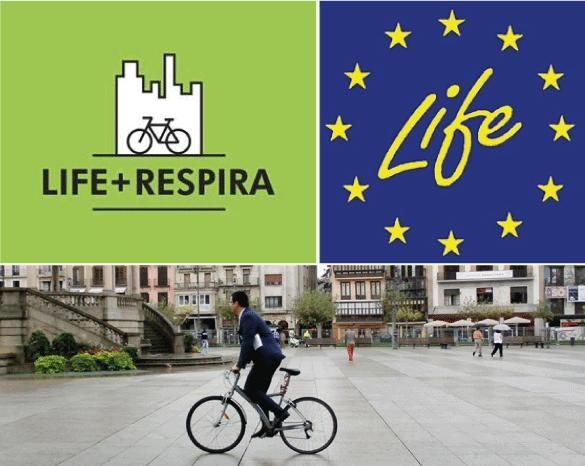
\includegraphics[width=\linewidth]{ lifeRespira.png}
    \caption{The announcement poster for the "Life+Respira" study}
    \label{chap:second:fig:1}
\end{figure}